\begin{refsection}
\chapter{Materials and Methods} % Main chapter title

\label{Chapter2} % Change X to a consecutive number; for referencing this chapter elsewhere, use \ref{ChapterX}

%\thispagestyle{empty}

%----------------------------------------------------------------------------------------
%	SECTION 1
%----------------------------------------------------------------------------------------

\section{Materials}

\subsection{Reagents for chromosomal analysis}
 \begin{sloppypar}\subsubsection{Roswell Park Memorial Institute 1640 (RPMI-1640): \textmd{Invitrogen (Cat. \# 23400-013)}} \end{sloppypar}
The contents of the RPMI 1640 powder was added to 950 mL of sterile water at room temperature (15°C to 30°C) water with gentle stirring. To this, 2 g of sodium bicarbonate was added the pH was adjusted to 0.2 and 0.3 units below the desired final working pH of 7 by slowly adding, with stirring, 1 N NaOH or 1 N HCl. To prevent microbial contamination, 100 μL of streptomycin, penicillin and gentamycin was added before the volume was made up to 1 L using sterile water. The prepared medium was then aliquoted immediately into sterile containers by membrane filtration with a 0.2-µm filter using a positive pressure system.
\subsubsection{Sodium bicarbonate: \textmd{HiMedia (Cat. \# TC230)}}
\subsubsection{Sodium hydroxide: \textmd{Qualigens (Cat. \# 15895)}}
\subsubsection{Hydrochloric acid: \textmd{Fischer (Cat. \# 29507)}}
\subsubsection{Fetal Bovine Serum (FBS): \textmd{Invitrogen (Cat. \#10270-106)}} 
\subsubsection{Phytohemagglutinin (PHA) : \textmd{Invitrogen (Cat. \#10576-015)}} 
\subsubsection{Ethidium bromide (1 mg/mL): \textmd{Sigma Aldrich (Cat. \# E7637)}}
To 10 mL of sterile double distilled water, 10 mg of ethidium bromide was added and mixed well for complete dissolution of the dye. The solution was stored at 4 °C.
\subsubsection{Colchicine (1 mg/mL): \textmd{HiMedia (Cat. \# RM342-10G)}}
To 10 mL of sterile double distilled water, 10 mg of colchicine was added and mixed well for complete dissolution. The solution was stored at 4 °C.


\subsubsection{Potassium chloride: \textmd{HiMedia (Cat. \# MB043)}}
To prepare a hypotonic solution (0.075 M), 0.56 g of potassium chloride was dissolved in 100 mL of distilled water and stored at room temperature. This was always pre-warmed prior to use.
\subsubsection{Carnoys Fixative}
Methanol (Fischer, Cat. \#16616) and glacial acetic acid (Merck Chemicals, Cat. \# 100063) were mixed in the ratio of 3: 1. The fixative solution was prepared fresh every day and pre-chilled prior to use.
\subsubsection{Phosphate buffer saline (PBS) (10X): \textmd{Nalgene (Cat. \# BP399-1)}}
\subsubsection{Trypsin from porcine pancreas: \textmd{ Sigma (Cat\# T4799-1G)}} 
Approximately 8 mg of trypsin was dissolved in 50 ml of 1X phosphate buffered saline (Invitrogen, Cat \# 14190250). The solution was always pre-warmed prior to use. 
\subsubsection{Giemsa staining solution: \textmd{HiTech Scientific Laboratories Pvt Ltd}}
Approximately 5 ml of Giemsa was dissolved in 45 ml of distilled water.
\subsubsection{Immersion Oil: \textmd{Himedia (Cat. \# GRM225)}}

\subsection{Reagents for FISH analysis of 22q11.2 microdeletion}
\subsubsection{Vysis DiGeorge Region Probe LSI \textit{TUPLE1} SpectrumOrange/LSI \textit{ARSA} SpectrumGreen Probe Kit: \textmd{Abbott Molecular Inc. (Cat. \# 08L59-020)}}
\begin{sloppypar}\subsubsection{Saline Sodium citrate (SSC) buffer: \textmd{Abbott Molecular Inc. (Cat. \# 02J10032)}}\end{sloppypar}

\subsubsection{Formaldehyde: \textmd{Qualigens (Cat. \# 12755)}}


\subsubsection{Formaldehyde fixation solution for FISH pretreatment}
1.3 mL of 37\% formaldehyde solution was mixed in 48.5 mL of PBS. 0.23 g of MgCl2 was added to the solution and mixed thoroughly. The working solution was stored at 4 °C.

\subsubsection{20X Saline sodium citrate} 
132 g of 20X SSC was thoroughly mixed in purified 400 mL purified water. pH was measured and adjusted to 5.3 with HCl. Purified water was added to bring the final volume up to 500 mL. The stock solution was stored at about 25 °C. 
\subsubsection{2X SSC solution for FISH pretreatment} 
100 mL of 20X SSC (pH 5.3) was mixed thoroughly with 850 mL of purified water. pH was measured and adjusted to 7.0±0.2 with NaOH. Purified water was added to bring the final volume up to 1 L. The solution was stored at about 25 °C.
\subsubsection{Pepsin: \textmd{Himedia (Cat. \# GRM1250)}}
\subsubsection{Pepsin solution for FISH pretreatment}
2.5 mg of lyophilized pepsin was mixed in 50 mL of 0.01 N HCl. The working solution was used immediately.
\begin{sloppypar}\subsubsection{Ethanol: \textmd{Changsu Yangyuan Chemicals (Cat. \# XK-13-201-00185)}} \end{sloppypar}
\subsubsection{Ethanol (70\%)}
70 mL of ethanol was diluted in 30 mL of sterile water and stored at about 25 °C.
\subsubsection{Ethanol (85\%)}
85 mL of ethanol was diluted in 15 mL of sterile water and stored at about 25 °C.
\begin{sloppypar}\subsubsection{IGEPAL CA-630 (Octylphenoxy poly(ethyleneoxy) ethanol): \textmd{Sigma Aldrich (Cat. \# I3021)}}\end{sloppypar}
\subsubsection{0.4X SSC/0.3\% IGEPAL solution for FISH post-hybridization wash}
1 mL of 20X SSC was mixed with 47 mL of distilled water. 150 µL of IGEPAL was added and thoroughly mixed until it dissolved completely. The pH was measured and adjusted to 7.0±0.2 with NaOH and was made up to the final volume of 50mL with distilled water. The solution was stored at about 25 °C.


\subsubsection{2X SSC/0.3\% IGEPAL solution for FISH post-hybridization wash}
5 mL of 20X SSC was mixed with 42 mL of distilled water. 50µL of IGEPAL was added and thoroughly mixed until it dissolved completely. pH was measured and adjusted to 7.0±0.2 with NaOH and was made upto final volume of 50mL with distilled water. The solution was stored at about 25 °C.
\subsubsection{4,6-Diamidino-2-phenyl indole (DAPI): \textmd{Abbott Molecular Inc. (Cat. \# 06J50-001)}}
\subsection{Reagents for  DNA extraction and qualitative analysis} 
\subsubsection{QIAamp® blood DNA mini kit: \textmd{Qiagen (Cat. \# 51104)}}
The kit provides the QIAamp spin column, collection tubes, Proteinase K, AL (lysis buffer for blood) ATL (lysis buffer for tissue) AW1 \& AW2 (wash buffers) and AE (elution buffers) 
\subsubsection{Tris Base: \textmd{Himedia (Cat. \# TC072)}}
\begin{sloppypar}\subsubsection{Ethylene diamine tetraacetic acid (EDTA disodium salt): \textmd{Merck (Cat. \#324503)}} \end{sloppypar}
\subsubsection{50X TAE buffer (Tris- acetate EDTA buffer)  (pH 7.2)}
\begin{itemize} 
\setlength{\itemindent}{+.5in}
\item Tris base : 2M
\item Glacial acetic acid: 1N
\item Na$_2$EDTA.2H$_2$O:  0.05M
\end{itemize}
	Tris base and disodium EDTA were dissolved in sterile double distilled water. Using glacial acetic acid, the pH was adjusted to 7.2. The final volume was made up to 1000 ml and sterilized by autoclaving. The solution was stored in a clean sterile reagent bottle at room temperature (25ºC) 
\subsubsection{Ficoll PM 400: \textmd{Sigma Aldrich (Cat. \# F4375)}}
\subsubsection{Bromophenol blue: \textmd{Himedia (Cat. \# MB123)}}
\subsubsection{Xylene Cyanol: \textmd{ Himedia (Cat. \# RM859)}}
\subsubsection{Tris HCl: \textmd{Himedia (Cat. \# TC073)}}
\subsubsection{6X DNA sample loading dye}
\begin{itemize} 
\setlength{\itemindent}{+.5in}
\item Ficoll PM 400 - 6\%
\item Bromophenol blue  - 0.12\%
\item Xylene cyanol  - 0.12\%
\item Tris- HCl (pH 7.5) - 12 mM
\item Na$_2$EDTA.2H$_2$O - 120 mM
\end{itemize}
All the components were dissolved in sterile double distilled water and stored at 25ºC.
\subsubsection{Agarose low EEO: \textmd{Bangalore Genei (Cat. \# 612600501001730)}} 
\subsection{Reagents for Polymerase chain reaction (PCR)}
\subsubsection{dNTP mix (10 mM): \textmd{Bangalore Genei (Cat. \# 610651200011730)}}
\subsubsection{Primers: \textmd{Shrimpex/Sigma}}
The lyophilized powders of different OD values were reconstituted with sterile water. The primer sequences for the selected genes of folate metabolism, \textit{TBX1} and \textit{NKX2.5} are specified in their respective chapters
\subsubsection{Taq DNA Polymerase (3 Units/μL): \textmd{Bangalore Genei (Cat \# 610602500\-051730)}}
\subsubsection{10X Taq DNA Polymerase Buffer: \textmd{Bangalore Genei (Cat \# 610602500\- 051730)}}
\subsubsection{Dimethyl sulfoxide (DMSO): \textmd{Sigma Aldrich (Cat. \# D8418)}}
\subsection{Reagents for Sanger DNA  sequencing and cycle sequencing} 
\subsubsection{BigDye® Terminator v1.1 Cycle Sequencing Kit: \textmd{Applied Biosystems (Cat. \# 4404307)}}
The kit comprises a 200µL tube of BigDye® Terminator v1.1 Ready Reaction Mix, a tube of M13 (-21) Primer, a tube of pGEM Control DNA and a 1mL tube of 5x Sequencing Buffer
\nopagebreak
\subsubsection{Hi-Di Formamide: \textmd{Applied Biosystems (Cat. \# 4404307)}}
\subsection{Reagents for RNA isolation from blood and tissue, cDNA conversion  and reverse transcriptase PCR (RT-PCR)}
\subsubsection{Ficoll histopaque: \textmd{Sigma Aldrich (Cat. \# 10771)}}
\subsubsection{Trizol:\textmd{Invitrogen (Cat. \# 15596-026)}}
\subsubsection{Chloroform: \textmd{Qualigens (Cat. \# 12305)}} 
\subsubsection{High capacity cDNA reverse transcription kit: \textmd{Applied Biosystems (Cat. \# 4368814)}}
The kit contains all components necessary for the quantitative conversion of up to 2 µg of total RNA to single-stranded cDNA in a 20 µL reaction which includes. 1 mL of 10X RT Buffer, 1 mL of 10X RT Random Primers, 0.2 mL of 25X dNTP Mix (100 mM) nd 0.2 mL of MultiScribe$^®$ Reverse Transcriptase (50 U/µL)

%\clearpage
%-----------------------------------
%	SECTION 2
%-----------------------------------

\section{Study population}
This was a case control study which included non-syndromic CTHD patients as the cases and healthy volunteers as controls .The cases and controls were similar in ethnicity, mainly from South India. An overview of the characteristic features of the study population is given in \cref{tab:2.1studypopulation}. The study was approved by Institutional Ethics Committee of Sri Ramachandra University, Chennai, India \textbf{(IEC- NI/09/DEC/13/38)}. 

%test table to change to original

\begin{table}[th]
\centering
\caption{Principal characteristics of the study population}
\label{tab:2.1studypopulation}
\begin{tabular}{  l  l  l  }
\hline
	Characteristics & Cases ( n=100) & Controls (n=100) \\ \hline
	Age, years (mean ± SD) & 6.51 ± 6.56 & 7.67 ± 5.32 \\ \hline
	Males & 61 & 49 \\ \hline
	Females & 39 & 51 \\ \hline
\end{tabular}
\end{table}

\subsection{Case group (n= 100)}
Individuals diagnosed with CTHD who fulfilled the following criteria were recruited:

\subsection{Inclusion criteria}
\begin{enumerate}
\item Age 0-18 years 
\item Males and females 
\item Diagnosed with structural abnormalities involving the outflow tract confirmed by a
pediatric cardiologist
\end{enumerate}
	
\subsection{Exclusion criteria}
\begin{enumerate}
\item Individuals with known genetic syndromes such as Down syndrome
\item Lack of consent
\end{enumerate}
	
The cases included are TOF, PTA, DORV, IGA and IAA.  The proportions of each subtype are provided in the \cref{fig:2_1casepopln}.

\begin{figure}[!b]
\centering
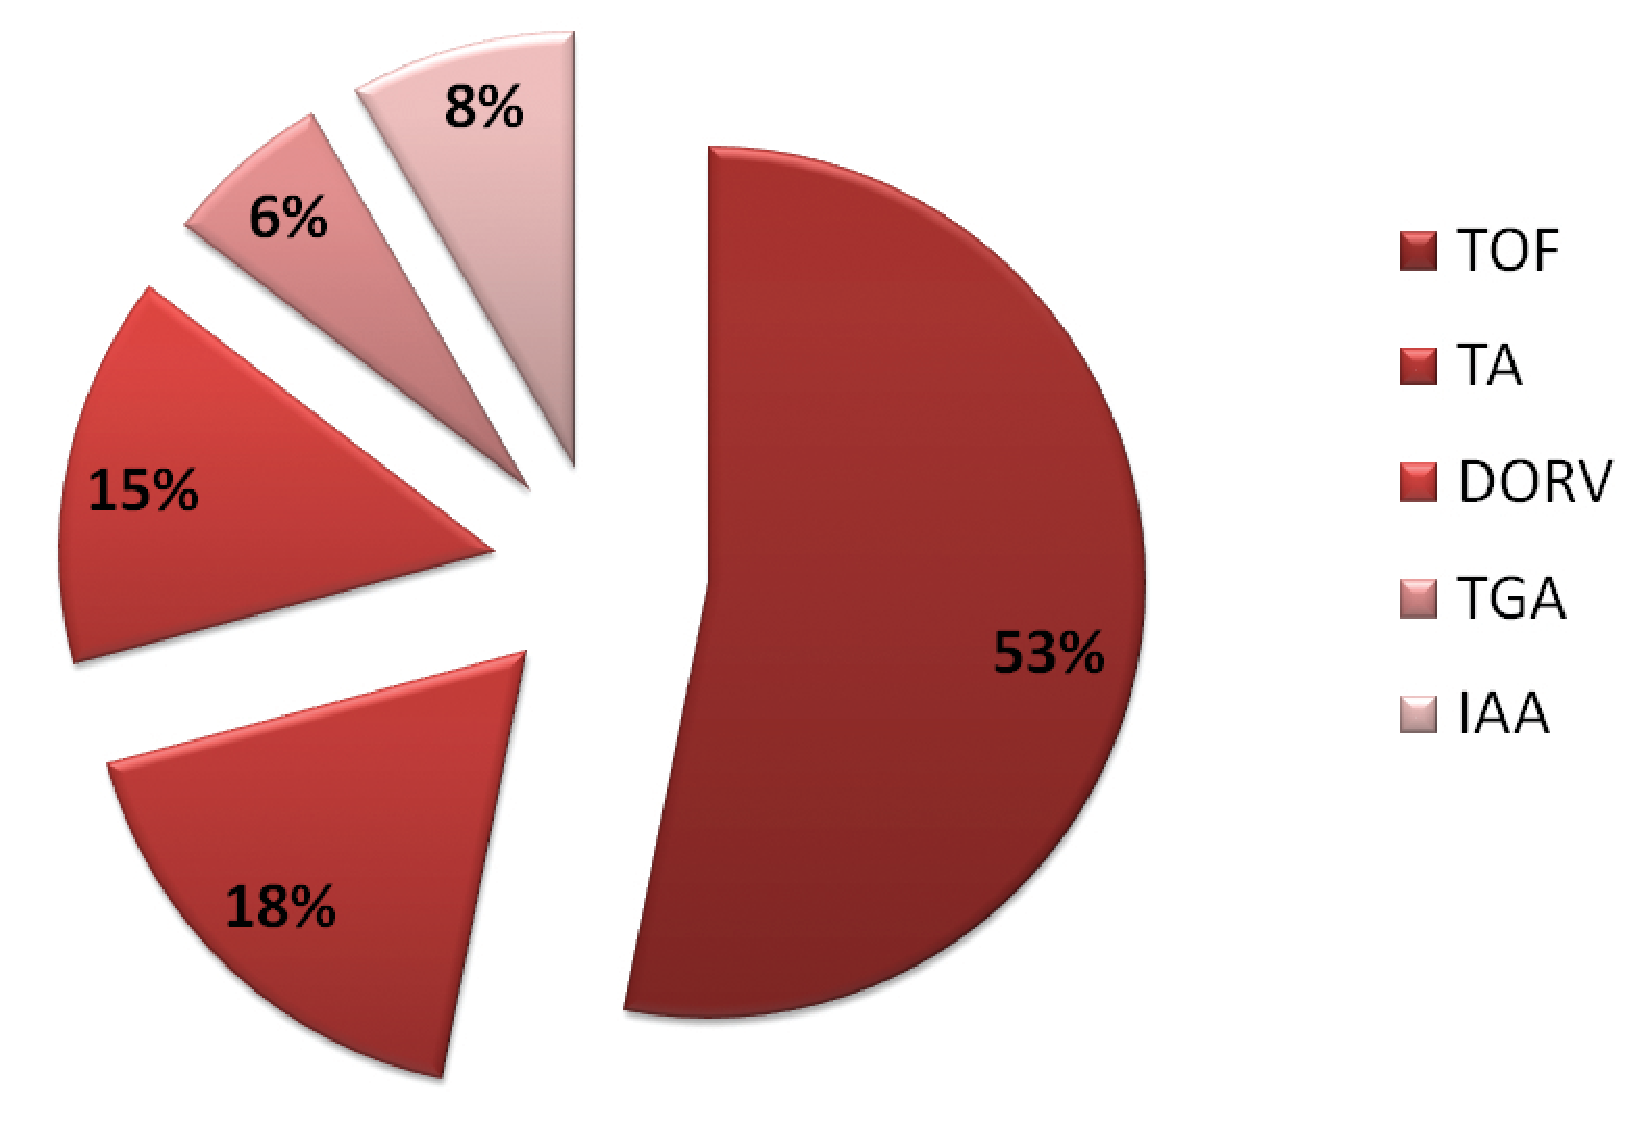
\includegraphics[scale=0.25,keepaspectratio]{Figures/2_1casepopln.pdf} 
\rule{35em}{0.5pt}
\caption{Distribution of CTHD in the case population}
\label{fig:2_1casepopln}
\end{figure}

\subsection{Control group (n= 100)}
This group comprised of age and gender matched healthy volunteers with no kinship to the cases and no history of genetic diseases or other birth defects, recruited from the same geographic area and time period as the cases. 


\subsection{Biological specimen collection}
2-3ml of venous blood was collected from all the participants. To analyze somatic mutations and the differential expression of \textit{NKX2.5} in the blood and tissue, surgical discards of the diseased heart was collected from of 55 of the cases. The biological specimens from both groups were collected from Sri Ramachandra Hospital and Madras Medical Mission, Chennai after obtaining an informed assent from a parent or guardian. 

\section{Methodology}

\subsection{Chromosomal analysis} 
Blood specimens were collected from CTHD cases and controls in sterile heparin vacutainers.
Chromosomal analysis was performed based on modified protocol described previously \cite{barch1997agt, moorhead1960chromosome, babu1995human, dracopoli1994current}.
\subsubsection{Culture initiation}
In a pre-labeled sterile 25 cm$^2$ culture flask, 8 ml RPMI medium, 2 ml FBS and 200 µl PHA was aliquoted followed by the addition of 1 ml of the blood sample. The contents were mixed well and incubated at 37°C and 5\% in a carbon dioxide (CO$_2$) incubator. The time of addition of PHA was considered the time of culture initiation and was noted as the zero hour.
\subsubsection{Metaphase arrest and lymphocyte harvesting}
At the 66½ hour after culture initiation 100 µl of ethidium bromide was added and the flask was incubated at 37°C for 30 minutes. At the 67\textsuperscript{th} hour, 100 µl of colchicine was added incubated at 37°C for a further 60 minutes. Thereafter, the contents were transferred to a clean 15 ml centrifuge tube, labeled appropriately. After centrifuging the contents at 1000rpm for 10 minutes and discarding the supernatant, 10ml of pre-warmed hypotonic solution was added, the contents mixed gently and then incubated at 37°C for 20 minutes. Following a second centrifugation at 1000rpm for 10 minutes and discarding the supernatant, approximately 8ml of pre-chilled carnoys fixative was added to the cell suspension while vortexing. Subsequent to 20 minute incubation at room temperature, the contents were once again centrifuged at 1000rpm for 10 minutes, the supernatant was removed and 10ml of fixative was added. The contents were kept at 4°C for 2 hours or until slide preparation. Before slide preparation, the cell pellet was washed with Carnoys fixative till a white cell pellet and a clear supernatant was obtained. Washing involved centrifugation at 1000rpm for 10 min, discarding the supernatant, addition of 10 ml of fresh fixative and vortexing to mix the contents.
\subsubsection{Slide preparation and Giemsa banding using trypsin and Giemsa (GTG)}
Slides were prepared by dropping an appropriately concentrated suspension of cells from an appropriate height onto clean, pre-chilled slides using a pasteur pipette. It was then placed on a hot plate, maintained at a temperature of 45-50°C, till it dried. The slide was then viewed under a phase contrast microscope and judged for chromosome spreading and adequate drying. Multiple slides were prepared from every sample for GTG-banding as well as FISH analysis. The slides aged overnight at 60°C were stained by GTG banding which involved mild agitation in an 16\%  trypsin solution for  approximately 8-10seconds , rinsing in 1 X PBS, staining in 10\% Giemsa stain for 4-6 minutes and a final rinse with distilled water. 
\subsubsection{Analysis}
For each case a minimum of 25 metaphases were analyzed for numerical and/or structural abnormalities. At least 5 metaphases were captured and karyotyped using the Cytovysion© karyotyping platform. All results were recorded as per the International System of Cytogenetic Nomenclature (ISCN) \cite{shaffer2013iscn}. Representative images of a normal female and male are presented in \cref{fig:2_2nmlfemale} and \cref{fig:2_3nmlmale}.

\begin{figure}[!tb]
\centering
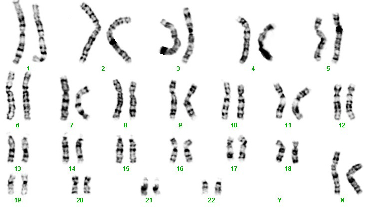
\includegraphics[width=\linewidth]{Figures/2_2nmlfemale.pdf} 
\rule{35em}{0.5pt}
\caption{Karyotype of a normal female: 46,XX (Case ID: CTHD004)}
\label{fig:2_2nmlfemale}
\end{figure}

\begin{figure}[!tb]
\centering
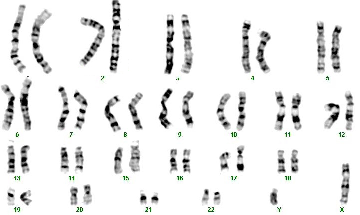
\includegraphics[width=\linewidth]{Figures/2_3nmlmale.pdf} 
\rule{35em}{0.5pt}
\caption{Karyotype of a normal male:46,XY (Case ID: CTHD007)}
\label{fig:2_3nmlmale}
\end{figure}

\subsection{Fluorescence In Situ Hybridization analysis}
FISH was performed to rule out the presence of the 22q11 microdeletion in the cases using the cell pellet of lymphocytes arrested in the metaphase
\subsubsection{Slide preparation and pretreatment}
Slides were prepared by dropping an appropriately concentrated suspension from an appropriate height onto clean, pre-chilled slides using a pasteur pipette. It was then placed on a hot plate, maintained at a temperature of 45-50°C, till it dried. The slide was then viewed under a phase contrast microscope and a 22 mm X 22 mm area having the maximum number of well spread metaphase plates was marked using a glass marker. The slides were aged at 90 °C for 1 hour and subsequently pretreated with pepsin to make the chromosomal DNA accessible for hybridization and to protect the morphology of the chromosomes from the denaturation process. The slides were incubated in 2X SSC solution at 37 °C for 1 hour and subsequently in pepsin solution at 37 °C for 13 minutes. Following this, the slides were washed in PBS, formaldehyde fixation solution and again in PBS at about 25 °C for 5 minutes each. Following air drying, the slides were dehydrated for 1 minute each in 70\%, 85\% and 100\% ethanol.
\subsubsection{Probe and target DNA co-denaturation and hybridization}
Approximately 2µl of the dual colour DiGeorge Region Probe-LSI \textit{TUPLE1} SpectrumOrange/LSI \textit{ARSA} SpectrumGreen probe in hybridization buffer was added to the marked area and then covered with coverslip that aided in the spreading of the probe. The sides of the coverslip were sealed using rubber cement and then placed in the HYBrite™ (Abbott Molecular), a hybridization chamber that allows for co-denaturation of the probe and target region and subsequent hybridization. The program parameters for these two processes were 73ºC for 5 minutes and 37ºC for 17 hours respectively.
\subsubsection{Post-hybridization washing}
After 17 hours, the coverslip is removed and the slide is gently agitated in 0.4X SSC/0.3\% IGEPAL wash solution at 70º±1C, for 30 seconds. Following which the slide was gently agitated in the 2X SSC/0.1\% IGEPAL wash solution at 37 °C for 30 seconds. While the slides were still damp 5 µl of the counterstain DAPI II was added, covered with a fresh coverslip and the sides sealed using nail varnish. The slides were stored at 4 °C for at least an hour before analysis.
\subsubsection{Analysis}
Using the Olypmpus BX-60 Fluorescent microscope, both interphase and metaphase chromosomes were analyzed for the presence of the normal number of fluorescent signals. A representative image is presented in \cref{fig:2_4fishcase}.

\begin{figure}[!tb]
\centering
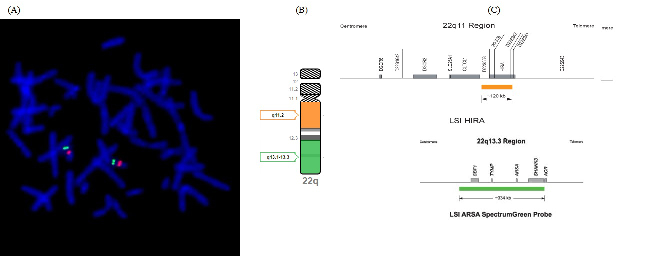
\includegraphics[width=\linewidth]{Figures/2_4fishcase.pdf} 
\rule{35em}{0.5pt}
\caption{(A) Representative metaphase of a case (Case \# CHD001) without the 22q11.2 microdeletion detected by FISH. The red signal indicates the 22q11.2 (TUPLE) region and the green signal the terminal chromosome 22 (\textit{ARSA}) region, used as control. (B) Schematic representation of chromosome 22. (C) Schematic representation of the probe map showing the usually deleted 3Mb region, the polymorphic DNA markers and the FISH probes used in this study.}
\label{fig:2_4fishcase}
\end{figure}

\subsection{Genomic DNA isolation from blood}
High molecular weight genomic DNA was isolated from the peripheral blood using the QIAamp® kit as per the manufacturer’s instruction. About 200 μl of blood was added to 20 μl of proteinase K and 200 μl of buffer AL in a 1.5 microcentrifuge tube. .The contents were briefly centrifuged and incubated at 55°C for 10 minutes. Subsequently 200 μl of 100\% ethanol was added and mixed again by pulse-vortexing for 15 seconds. The mixture was carefully applied to the QIAamp mini spin column without wetting the rim and centrifuged at 8000 rpm for 1 minute. The QIAamp Mini spin column was placed in a clean 2 ml collection tube, and the tube containing the filtrate was discarded. Then 500 μl of buffer AW1 and AW2 was added sequentially and centrifuged at 8000 rpm for 1 minute. Finally, the DNA was eluted in 200 μl of AE buffer into a collection tube. The DNA eluted was stored at -50 °C until use in experiments
 
\subsection{Genomic DNA isolation from tissue}
The cardiac tissue was mechanically homogenized using a mortar and pestle and transferred to a 1.5ml microcentrifuge tube. After adding 100 μl of ATL buffer and 20 μl of proteinase K it was mixed by vortexing, and incubated at 56°C. At the end of 2 hours, 200 µl buffer AL was added to the sample, mixed by pulse-vortexing for 15 s, and incubated at 70°C for 10 min. Subsequently 200 μl of 100\% ethanol was added and mixed again by pulse-vortexing for 15 s. Then the remaining steps were similar to that of DNA isolation from the blood tissue; thus the DNA was eluted in 200 μl of AE buffer and stored at -50 °C until use in experiments. 
\subsection{Qualitative and quantitative analysis of DNA}
\subsubsection{Agarose gel electrophoresis}
The quality of the isolated DNA was checked in a 0.8\% agarose gel. About 0.8 g of agarose was dissolved in 100ml of 1X TAE buffer by boiling. The solution was allowed to become lukewarm followed by which ethidium bromide was added to a final concentration of 0.1 mg/ml. The gel was then poured on a gel-casting tray and allowed to solidify and placed in an electrophoresis tank with 1X TAE buffer. The DNA samples were mixed with 6X bromophenol blue dye, loaded into the wells and electrophoresed at 2 volts/cm. The gels visualized in a gel documentation system (Bio Rad) and the quality of DNA was interpreted based on the band intensity as observed in \cref{fig:2_5DNAqlty}A.
\subsubsection{Analysis using the nanodrop} 
The quantity of the DNA specimens were assessed using the nanodrop based on the ratio of absorbance at 260 nm and 280 nm. About 2 µl of the DNA was added to the lower pedestal of the nanodrop and the assessment of the purity of DNA was made. A ratio of ~1.8 was generally accepted as a good quality DNA (\cref{fig:2_5DNAqlty}B).

\begin{figure}[!tb]
\centering
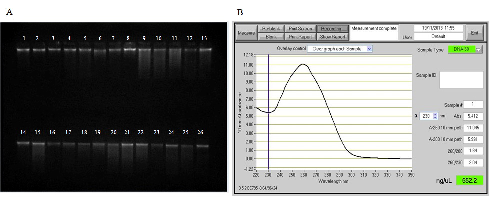
\includegraphics[width=\linewidth]{Figures/2_5DNAqlty.pdf} 
\rule{35em}{0.5pt}
\caption{(A) Quality of DNA extracted from the blood (Lane 1-13) and tissue (Lane 14-26)  as observed as good; as displayed on 0.8\% agarose electrophoresis stained with ethidium bromide. The band intensity depends on the DNA concentration. (B) Nanodrop sample output measurement for the DNA isolated from case (Case ID: CHD005)}
\label{fig:2_5DNAqlty}
\end{figure}

\subsection{Polymerase chain reaction (PCR)}
Amplification of the gene of interest rs1801133, rs1801131, rs1051266, rs1805087, rs1801394  rs1532268, \textit{TBX1} and \textit{NKX2.5} was performed using specific primers under appropriate cycling conditions of denaturation, annealing and extension in a Thermal cycler (Master Cycler gradient- Eppendorf).

The PCR was performed in 20µl reactions with a master mix comprising of all the components listed in \cref{tab:2.2pcrmm}, except the template, was prepared and aliquoted into separate tubes. The template DNA was then added; the tubes were placed in the thermal cycler and subjected to the standardized PCR conditions. The PCR conditions were standardized for each gene by gradient PCR. While the annealing temperature and time differed for the each of the genes in this study, the remaining PCR conditions were constant and are given in \cref{fig:2_6pcrconditions}. The presence of amplicons was confirmed by 2\% agarose gel electrophoresis. A 100 bp DNA molecular weight marker was used confirm the amplicon size. Electrophoresis was carried out at 4V/cm and the gel was visualized in the gel documentation system. The representative gel images are presented in the respective chapters.

\begin{figure}[!tb]
\centering
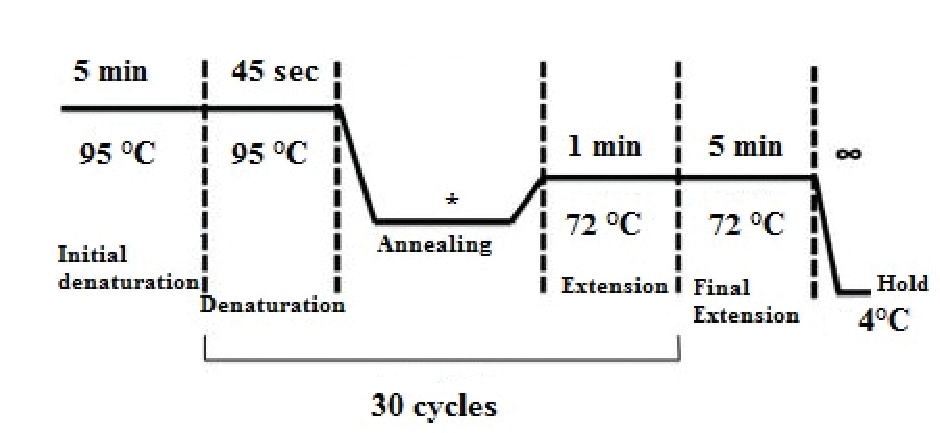
\includegraphics[width=\linewidth]{Figures/2_6pcrconditions.pdf} 
\rule{35em}{0.5pt}
\caption{Standard PCR conditions: The reaction conditions of the PCR amplification are composed of the total number of cycles to be run and the temperature and duration of each step in those cycle. The annealing temperature (*) is based on the Tm of the primer pair and ranges from 50–68°C for the primers used in this study. \cite{Cabuk2007, deeparani2009detection, galbiatti20105, zeng2011a66g, goldmuntz2001nkx2}}
\label{fig:2_6pcrconditions}
\end{figure}

\begin{table}[!h]
\centering
\caption{Components of a PCR mastermix}
\label{tab:2.2pcrmm}
\begin{tabular}{  l  l  l  }
\hline
	Reagents & Working Concentration & Reaction Volume (μL) \\ \hline
	PCR Buffer & 1X & 2 \\ \hline
	dNTPs & 200μM & 0.4 \\ \hline
	Forward Primer & 50pM & 0.2 \\ \hline
	Reverse Primer & 350pM & 0.2 \\ \hline
	Taq Polymerase & 1.5 Units & 0.5 \\ \hline
	Template DNA & 100ng & 2 \\ \hline
	Nuclease-free water &  & 14.5 \\ \hline
\end{tabular}
\end{table}

\subsection{DNA sequencing} 
The amplified product of the respective genes was sequenced in two steps; a sequencing PCR followed by post PCR processing and sequencing.  Bi-directional sequencing PCR was performed with the amplicon as the template, with the respective forward or reverse primers (\cref{tab:2.3cycseqmm}) and then dispensed equally into microAmp 96well plate. The amplicons were then added to the wells and subjected to sequencing PCR reaction which is outlined in \cref{fig:2_7cycseqconditions}.

\begin{figure}[!b]
\centering
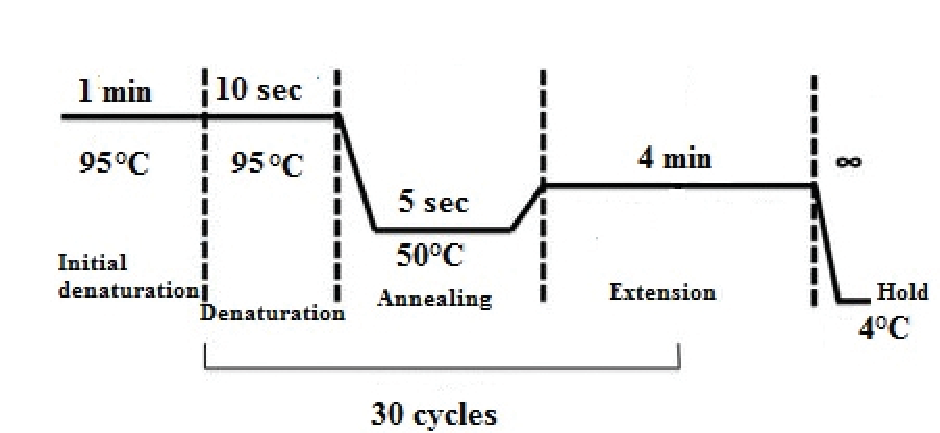
\includegraphics[width=\linewidth]{Figures/2_7cycseqconditions.pdf} 
\rule{35em}{0.5pt}
\caption{Cycle sequencing conditions: The reaction conditions are similar to standard PCR except there is one primer added to the reaction and successive rounds of denaturation, annealing, and extension in a thermal cycler result in linear amplification of a single stranded DNA where terminal nucleotide is labeled with a fluorescent dye.}
\label{fig:2_7cycseqconditions}
\end{figure}

For the post processing purification 20 μl of EDTA, followed by 30 μl of 100\% ethanol was added to each well containing products of the cycle sequencing. The plate was incubated at 370C for 10 minutes, and spun at 3600rpm for 30 minutes. A pop spin was given at 200rpm for 5 seconds, following which, 25 μl of 70\% ethanol was added to the wells. The plate was then spun at 3600 rpm for 5 minutes, followed by a second pop spin. After air- drying, 10 μl of Hi-Di formamide was added and the plate was linked for sequencing to the Genetic Analyzer 3730 (Applied Biosystem, UK). 

\begin{table}[!h]
\centering
\caption{Cycle sequencing PCR reaction mix}
\label{tab:2.3cycseqmm}
\begin{tabular}{  l  l  }
\hline
	Reagents           & Volume (μl) \\ \hline
	BigDye™ & 0.5 \\ \hline
	5X BigDye™ buffer & 1.5 \\ \hline
	Forward / Reverse Primer & 0.5 \\ \hline
	DNA template & 2 \\ \hline
	Sterile water & 5.5 \\ \hline
\end{tabular}
\end{table}

The sequences obtained were then analyzed using two software; Chromas for single nucleotide polymorphisms and SeqScape analysis software V2.5. for mutation analysis as presented in \cref{fig:2_8chromatogram}. 

\begin{figure}[!tb]
\centering
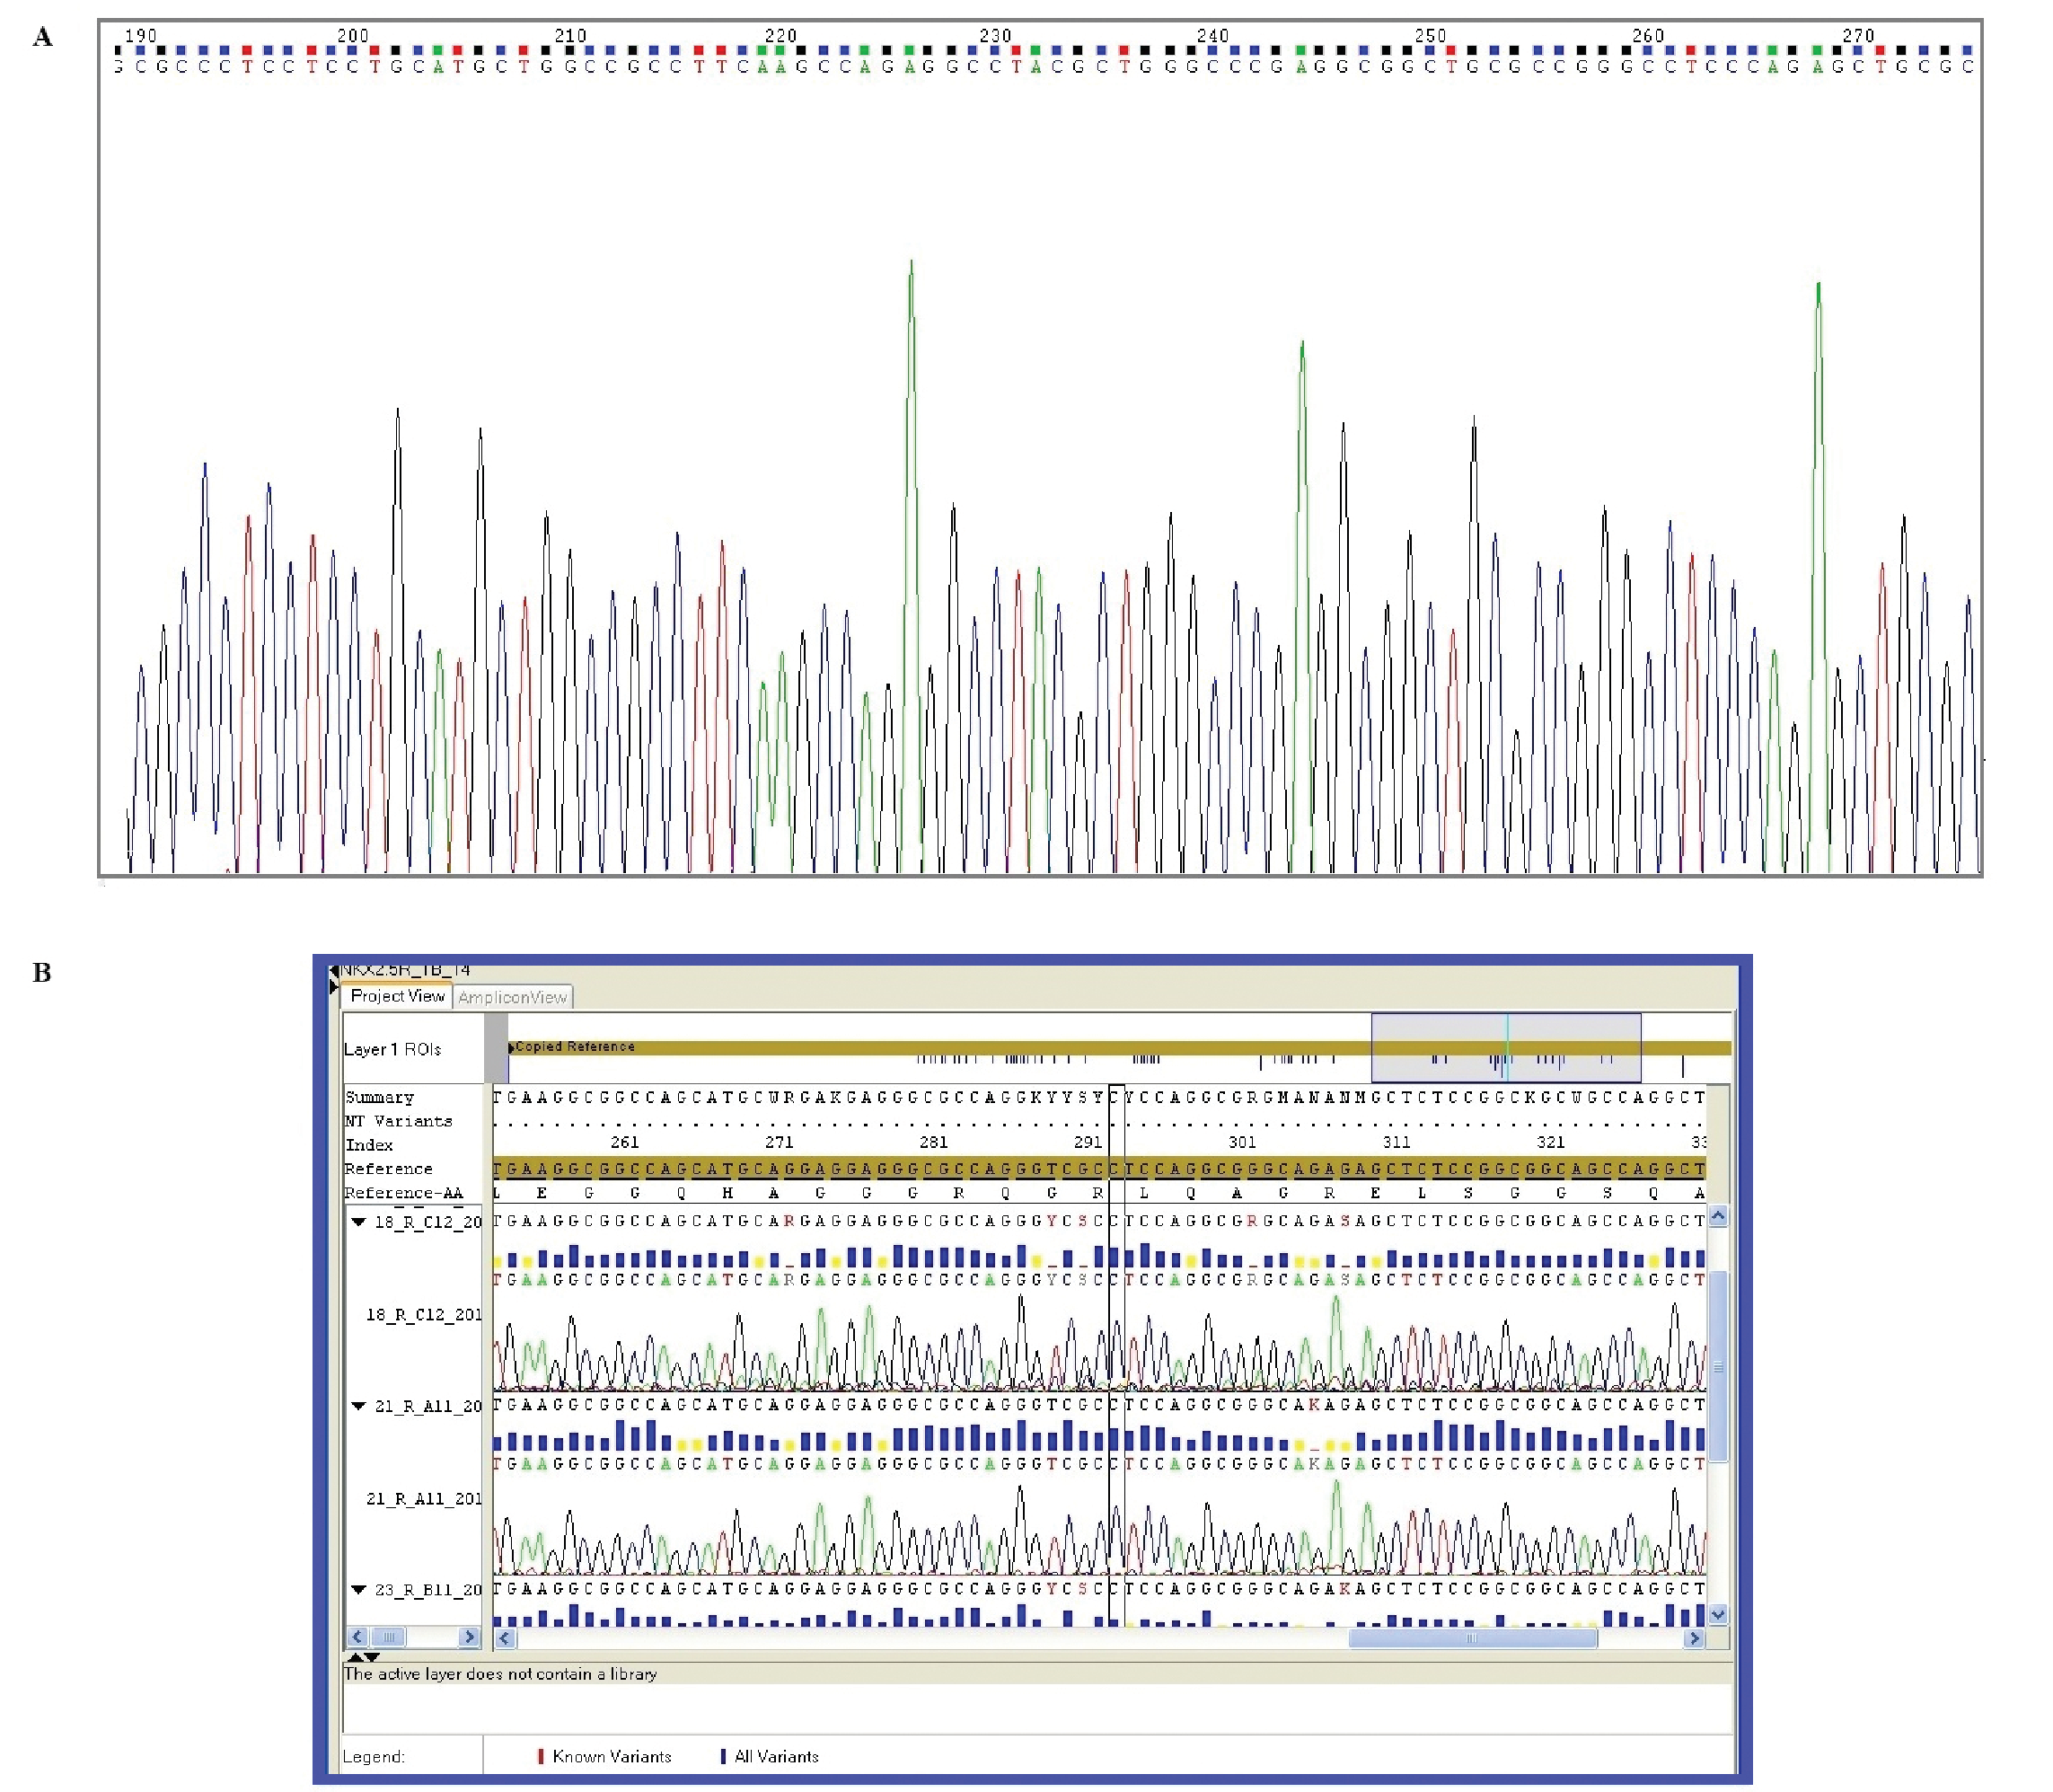
\includegraphics[width=\linewidth]{Figures/2_8chromatogram.pdf} 
\rule{35em}{0.5pt}
\caption{(A) Sequence chromatograms of \textit{NKX2.5} (B) Seqscape (Ver 2.9)analysis of \textit{NKX2.5} mutations  that allows for alignment of multiple sequence chromatograms  with the reference gene sequence so that point mutations can be detected simultaneously.}
\label{fig:2_8chromatogram}
\end{figure}

\subsection{RNA isolation and cDNA conversion from tissue and blood} 
About 10 mg of cardiac tissue was ground in 1 ml of trizol reagent using a sterile mortar and pestle. The resulting suspension was transferred to a 2 ml microfuge tube and the mixture was incubated for 10 minutes. Whereas, in blood samples, the white blood cells (WBC) were isolated in Ficoll-histopaque density gradient centrifugation medium  and  re-suspended in trizol reagent. For both the tissue and WBC suspended in the trizol, 200 μl of chloroform was added and incubated for 10 minutes. The tubes were then spun at 10,000rpm for 10 minutes. The top phase was transferred to a fresh 1.5 ml microcentrifuge tube and 500 μl of 70\% ethanol was added to it. The mixture was spun down and the supernatant was discarded. The pellet was allowed to dry and was suspended in 20μl of sterile water. 

All the RNA samples were adjusted to the equal concentration before proceeding to cDNA synthesis. A 10µl reaction was set up (composition as given in \cref{tab:2.4cdnamm}) using 10µl of 2 X RT master mixes was added and 10µl of total RNA in a clean sterile PCR tube. The tube was placed inside master cycler PCR and amplified using the program as given below in \cref{tab:2.5cdnaprog}. The cDNA was then stored at -20°C until further processing in a clean sterile PCR tube. 

\begin{table}[!tb]
\centering
\caption{Mastermix for cDNA synthesis}
\label{tab:2.4cdnamm}
\begin{tabular}{  l  l  }
\hline
	Reagents & Volume/reaction (µl) \\ \hline
	10X RT Buffer & 2 \\ \hline
	10X Random Primers & 2 \\ \hline
	25X dNTP (100mM) & 0.8 \\ \hline
	Multi-scribe RT enzyme & 1 \\ \hline
	Sterile water & 4.2 \\ \hline
\end{tabular}
\end{table}



\subsection{RT-PCR}
RT-PCR was performed in the thermocycler (9700 HT RT-PCR, Applied Biosystem, UK) using SYBR green chemistry. A master mix comprising of all components except the template was prepared as given in \cref{tab:2.6rtmm} and aliquoted into separate tubes. 

\begin{table}[!tb]
\centering
\caption{Program for cDNA synthesis}
\label{tab:2.5cdnaprog}
\begin{tabular}{  l  l  l  l  l  }
\hline
	Temperature & 25 & 37 & 85 & 4 \\ \hline
	Time & 10 minutes & 120 minutes & 5 seconds & ∞ \\ \hline
\end{tabular}
\end{table}

\begin{table}[!h]
\centering
\caption{Preparation of Real Time PCR Reaction Mixture}
\label{tab:2.6rtmm}
\begin{tabular}{  l  l  }
\hline
	Reagents & Volume (μl/reaction) \\ \hline
	SYBR Green & 2.5 \\ \hline
	Forward Primer & 0.15 \\ \hline
	Reverse Primer & 0.15 \\ \hline
	cDNA (1:50 dilution) & 2 \\ \hline
	Water & 0.2 \\ \hline
\end{tabular}
\end{table}

The template was then added and the tubes were placed in the thermal cycler and subjected to PCR conditions with  initial temperature of 55°C for 10 minutes and a hold temperature of 95°C for SYBR green activation followed by denaturation and annealing temperatures of 55C for 1 min. Negative controls without cDNA were also performed. A melting curve analysis was made after each run to ensure a single amplified product for every reaction. The amount of target gene, normalized to an endogenous control β-actin was determined by the delta C$_t$ method.

\clearpage
\printbibliography[heading=subbibintoc]
\end{refsection}
